\usetikzlibrary{shapes,arrows}
\tikzstyle{block} = [draw, fill=blue!20, rectangle, 
    minimum height=2em, minimum width=4em]
\tikzstyle{sum} = [draw, fill=blue!20, circle, node distance=1cm]
\tikzstyle{input} = [coordinate]
\tikzstyle{output} = [coordinate]
\tikzstyle{pinstyle} = [pin edge={to-,thin,black}]
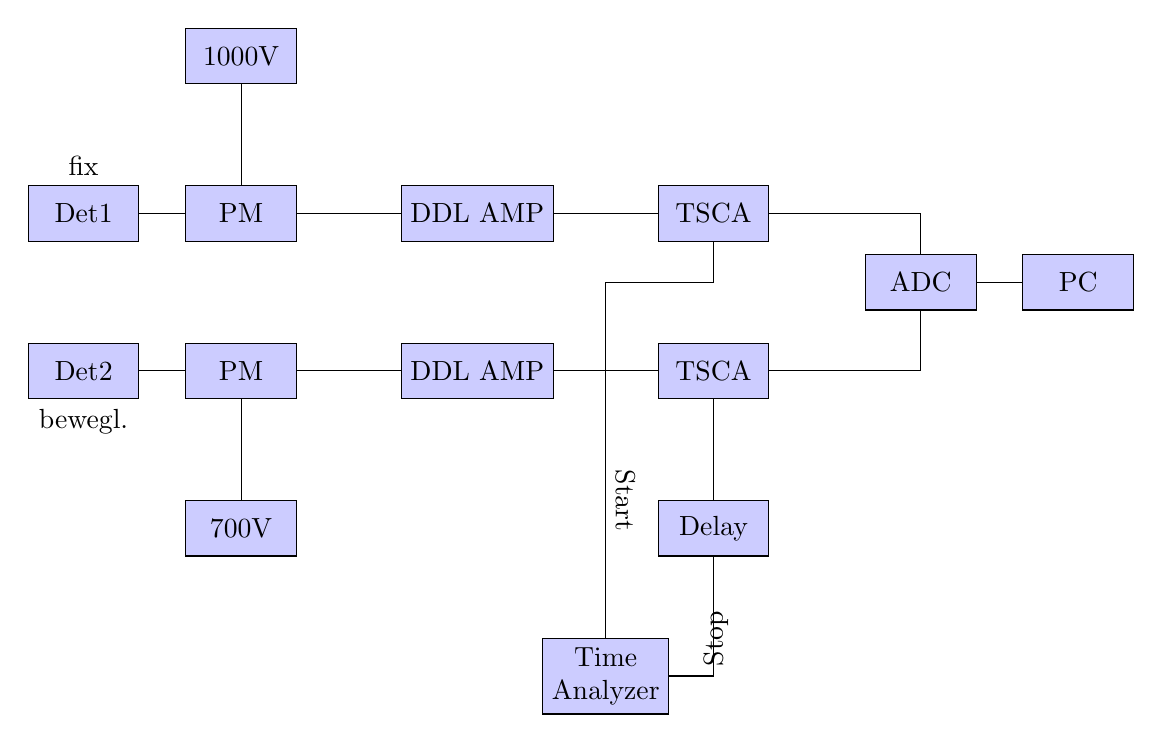
\begin{tikzpicture}[auto, node distance=2cm]

\node  [block, name=det1, label={[]above:fix}] {Det1};
\node [block, right of= det1] (pm1) {PM};
\node [block, below of=det1, name=det2,  label={[]below:bewegl.}] {Det2};
\node [block, right of= det2] (pm2) {PM};
\node [block, above of=pm1, name=volt1] {1000V};
\node [block, below of=pm2, name=volt2] {700V};

\draw [-] (det1) -- node[] {} (pm1);
\draw [-] (det2) -- node[] {} (pm2);
\draw [-] (volt1) -- node[] {} (pm1);
\draw [-] (volt2) -- node[] {} (pm2);

\node [block, name=ddl1, right of=pm1, node distance=3cm] {DDL AMP};
\node [block, name=ddl2, right of=pm2, node distance=3cm] {DDL AMP};
\node [block, name=tsca1, right of=ddl1, node distance=3cm] {TSCA};
\node [block, name=tsca2, right of=ddl2, node distance=3cm] {TSCA};

\draw [-] (pm1) -- node[] {} (ddl1);
\draw [-] (ddl1) -- node[] {} (tsca1);
\draw [-] (pm2) -- node[] {} (ddl2);
\draw [-] (ddl2) -- node[name=line1] {} (tsca2);

\node [block, name=time, below of=line1, node distance=4cm, align=center]{Time\\ Analyzer};
\node [input, name=node1, above of=line1, node distance=1cm] {};
\draw[-] (tsca1) |- node[] {} (node1) -- node[label={[rotate=-90, text depth=-6ex]right: Start}]{} (time);
\node [block, name=delay, below of=tsca2]{Delay};
\draw[-] (time) -| node[label={[rotate=90, text depth=-3ex]right:Stop}]{} (delay);
\draw[-] (delay) -- node[]{} (tsca2);

\node[block, name=adc, right of=node1, node distance=4cm] {ADC};
\draw[-] (tsca1) -| node[]{} (adc);
\draw[-] (tsca2) -| node[]{} (adc);
\node [block, name=pc, right of=adc]{PC};
\draw[-] (adc) -- node[]{} (pc);

\end{tikzpicture}